    \subsubsection{Tableau des scores}
    \begin{frame}{comparaison des scores}
           
    \end{frame}
    
    \begin{frame}
        les Graphiques suivant montre plusieures représentations des résidus des deux modèles 
    \end{frame}
    \begin{frame}{Lasso}
        \begin{center}
            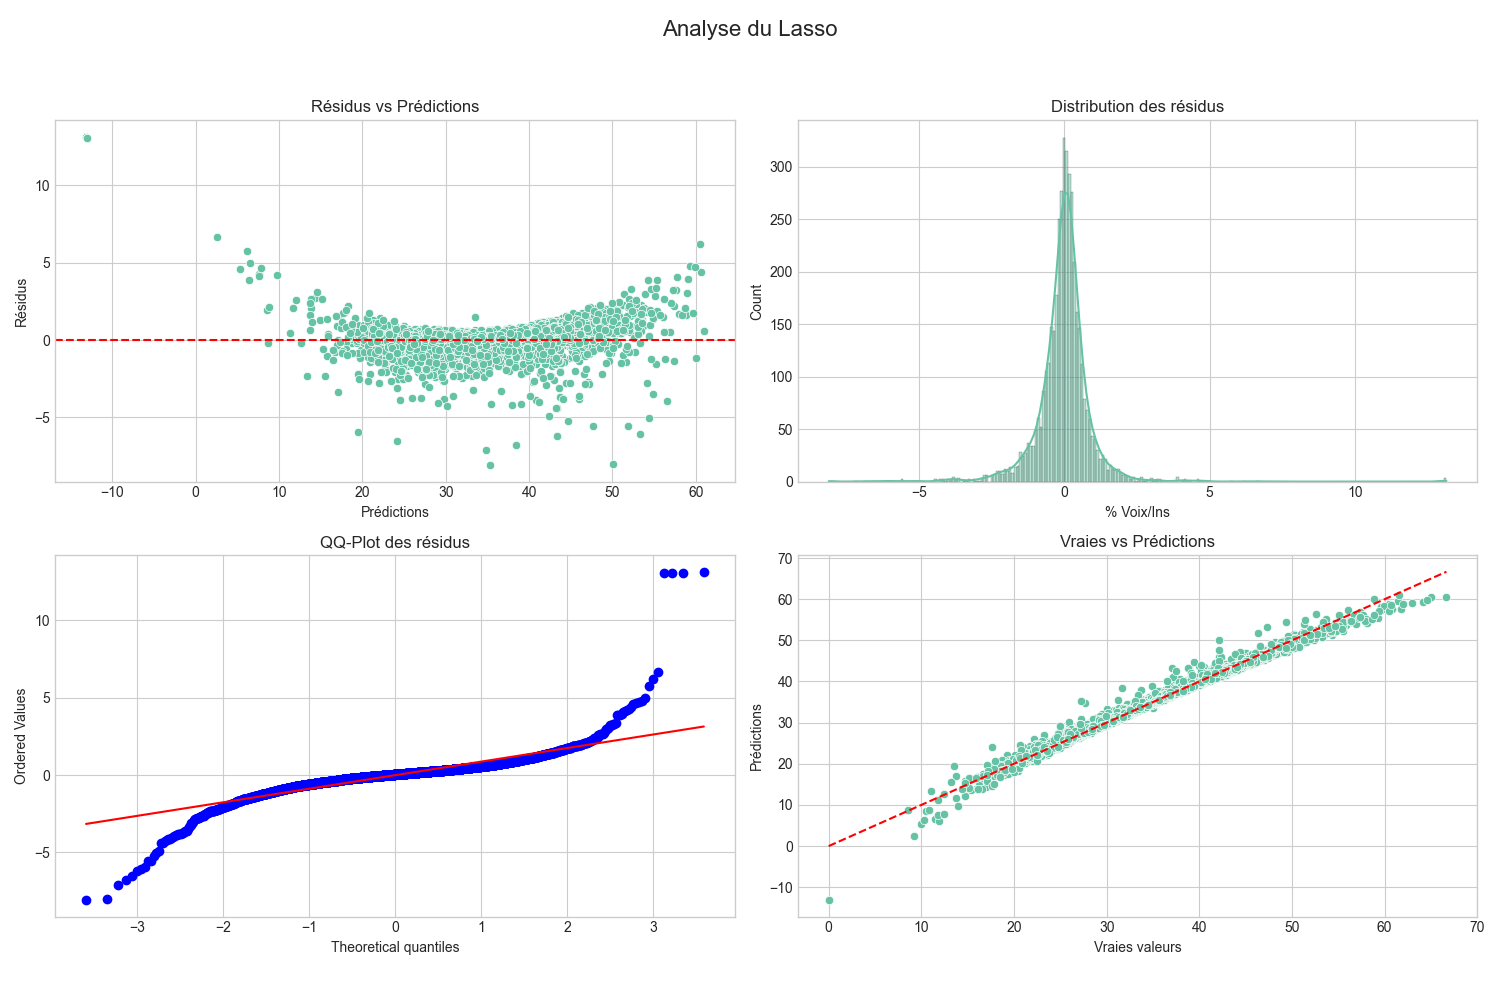
\includegraphics[width=0.8\textwidth]{figures/graphs_analyse_model_Lasso.png}
        \end{center}
    
    \end{frame} 

              
        
    \begin{frame}{XGBoost}
        \begin{center}
            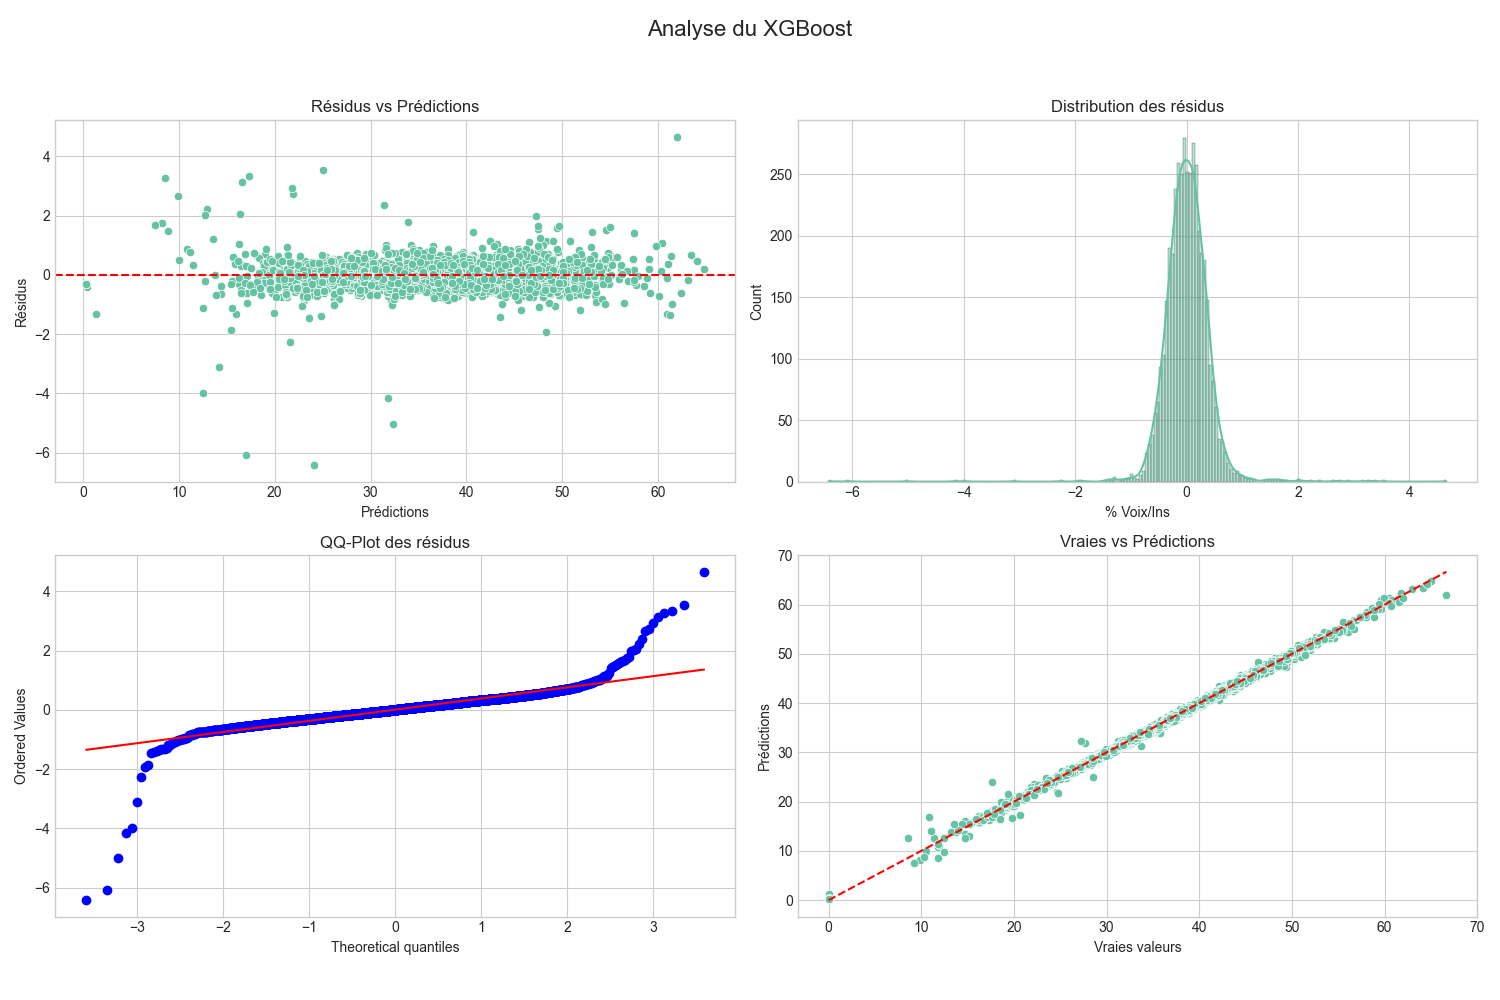
\includegraphics[width=0.8\textwidth]{figures/graphs_analyse_model_XGBoost.png}
        \end{center}
    
    \end{frame}    
        


\begin{frame}[allowframebreaks]{Interprétation des graphiques}
    
    les QQ-plots des résidus :  vus qu'ils représentent les quantiles d'une distribution normale théorique vs ceux observés , et comme les deux modèles ont des courbes en 'S' très applaties et presque centrée sur la diagonale , ont en conclut que 'les résidus des deux modèles on une distribution  presque normale '
                
    \framebreak        
    Histogrames des résidus : la différence notable , ce sont l'intervalles sur lesquels ils s'étalent :
        \begin{itemize}
            \item[.] ceux de XGBoost s'étalent de -6 à 6
            \item[.] ceux de Lasso s'étalent de -11 à 11
        \end{itemize}

        cela veut dire que les erreurs de Lasso varient beaucoup (prennent des valeurs plus ) plus que ceux de XGBoost , donc XGBoost est préférable comme modèle

    \framebreak

    \textbf{ Residus vs Prédictions} : les graphiques montres que les residus de XGBoost sont plus concentrés autour de zero que ceux de Lasso . On ve
    
    \framebreak

    \textbf{}
\end{frame}
